%!TEX root = Lefley - Mesh to voxel transformations for optimised physics-based interactions.tex
\chapter{Introduction}

\section{Motivation}

Physics simulation is one of the key components of a modern game engine. The more accurate the simulation is, the more immersive games built with the engine are likely to be. If the world around the player does not react as expected then it is difficult to become immersed in the game environment.

\section{Problem}

\label{sect:prob}

The most common representation of a solid object in a physical simulation is a rigid polygonal mesh. This format stores the vertices and faces which define the object's surface, with volume information being implicit. This is optimal for operations which require only the surface information, such as rendering, but presents issues if we wish to reason on the object's interior, as we do when fragmenting under physical forces.

It is possible to fragment an object without knowledge of its interior by simply partitioning the space in which the object exists and refining any partitions which have faces in them. However, as no volumetric information about the object is being used, the fracturing is approximate. A further limitation is that most implementations using similar approaches are restricted to convex objects or must first decompose any concave objects into constituent convex meshes~\cite{Muller:2013:RTD:2461912.2461934}.

Overall, while fragmentation from only surface information is efficient and produces reasonable results, the physical accuracy is limited and this project instead proposes a method which uses the object's volumetric information.

\section{Solution}

\label{sect:sol}

Taking an object as a three dimensional scalar field of mass, we simplify the problem of fragmenting it on the applied physical forces. For each point inside the object we determine which fragment that point should belong to based on the object's physical properties.

When only the boundary is stored, determining whether any given point is inside of an object is non trivial. Consider a series of faces defining a 2D object. Then to label any given point as inside the object we need to check that it is `inside' of all of the faces\cite{Ray-tracing}. Furthermore, this only holds for convex shapes, if there exist any concave sections then we could have a point which is `outside' of a face but inside the 2D object. See Figure~\ref{fig:1.1}.

\begin{figure}[b!]
\centerline{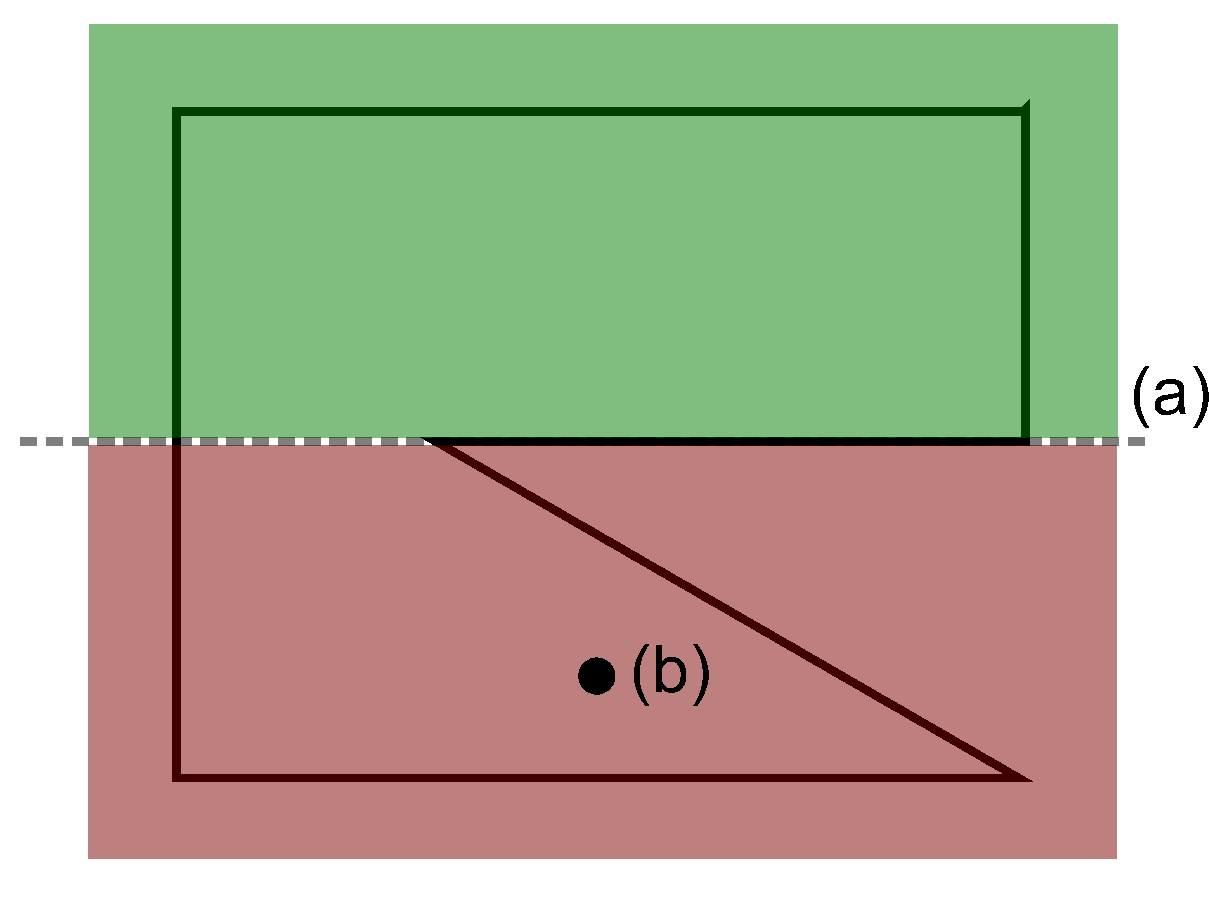
\includegraphics[scale=0.4]{point_inside_concave13.pdf}}
\caption{The green area shows all points `inside' line (a). The red areas shows all points `outside' line (a). Point (b) is `outside' line (a) but inside the defined concave shape.}
\label{fig:1.1}
\end{figure}

Calculating for all points, whether they are inside the object before physical interaction can reduce the simulation time complexity discussed above. We also gain a constant time lookup for checking if any given point lies within the object. This process is known as binary solid voxelisation, where a binary voxel is a point in three dimensional space with an assignment based on whether it is inside or outside of a given object\cite{Schwarz:2010:Vox}.

This project proposes a pipeline for simulating physical destruction, focussing on fragmentation, consisting of the following stages.
\begin{enumerate}
\item{Objects are voxelised}
\item{Each voxel is assigned to a fragment algorithmically in such a way as to emulate the physical properties of the object}
\item{A rigid mesh is built for each fragment from its constituent voxels}
\end{enumerate}

For example, if a bullet is fired at a brick wall, both the bullet and wall will be rigid meshes when the bullet is shot. On collision, both the wall and bullet will be voxelised. Assuming the bullet consists of only one voxel, no destruction calculations will be performed on it. Using the force of impact and physical parameters of the wall, it will be calculated which voxels should belong to which fragments. These fragments will then be transformed back into rigid meshes and the correct movement vectors will be applied. This is illustrated in Figure~\ref{fig:1.2}.

\begin{figure}
\centerline{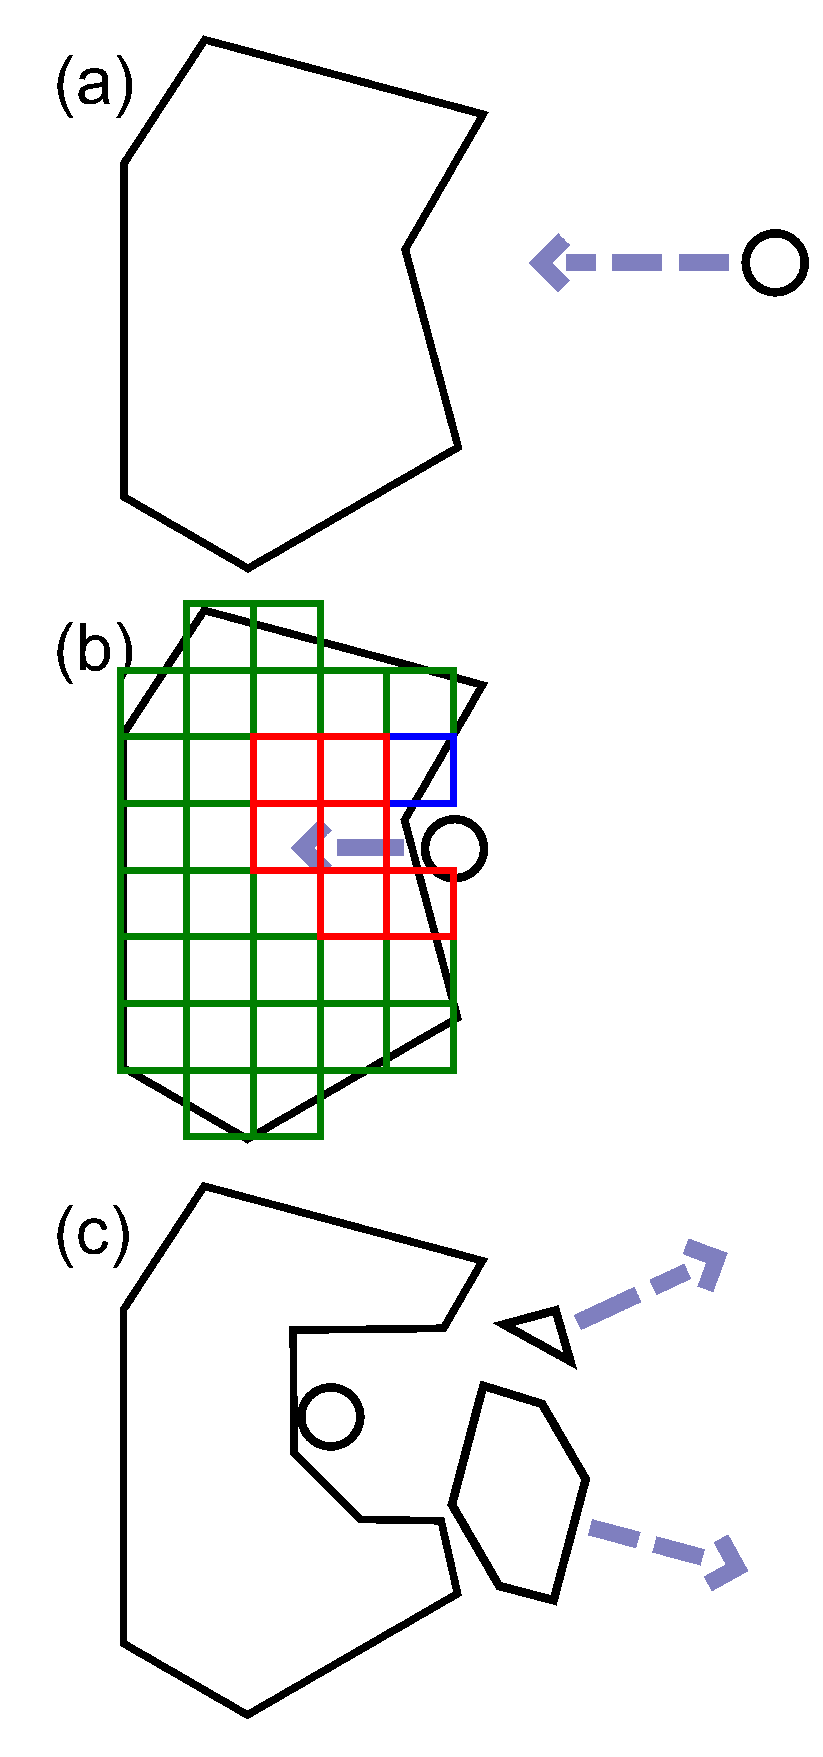
\includegraphics[scale=0.6]{diagram13.pdf}}
\caption{A simple rigid mesh projectile is fired towards another rigid mesh (a). On collision the destructible body is voxelised (b) depending on the force of the projectile and physical parameters of the objects. It is determined which voxels will detach, shown in red. Meshes are reformed around all separate bodies and physical forces are applied (c).}
\label{fig:1.2}
\end{figure}

This process will be referred to as {\emph{Dynamic Volumetric Fragmentation (DVF)}}.

\section{Related Work}

\subsection{Fragmentation}

\label{sect:relfrag}

One existing method for object destruction is a static approach. Fragments are generated for every destructible object when the objects are created and then substituted for the object on collision. This does not allow the result of the collision to be in any way dependant on the forces involved in the collision and so does not produce realistic results.

Matthias M\"{u}ller, Nuttapong Chentanez and Tae-Yong Kim propose a method for the dynamic destruction of objects in real time. The method uses `volume approximate convex decompositions' to fragment objects which are composed of convex pieces using Voronoi decomposition of space\cite{Muller:2013:RTD:2461912.2461934}.

\subsection{Mesh/Voxel Conversion}

Binary voxelisation of polygonal objects is a memory efficient method for defining occupied space and can be achieved in real-time on modern GPUs. Both surface and solid voxelisation methods are presented by Schwarz and Seidel\cite{Schwarz:2010:Vox}. A solid voxelisation algorithm was used as opposed to surface voxelisation as the entire volume of an object is required for the proposed volumetric destruction.

Both marching tetrahedra and surface nets exist as algorithms for constructing 3D surfaces from volumetric data\cite{Tetrahedra}\cite{Gibson:1998:CES:646921.709482}. An existing implementation of marching tetrahedra has been used as part of the remeshing stage of the pipeline as more literature existed concerning the use of this method with Unity3D\cite{Tetrahedra-CPU}.

\subsection{Related Uses}

Nie\ss{}ner et al present a method for real-time collision detection of patch based objects using mesh to voxel transformations \cite{niessner2013collision}. While their work is on collision detection, it does demonstrate that real-time mesh to voxel conversion is viable for use in resolving physics interactions.

Miguel Cepero is developing a procedural voxel engine Voxel Farm\cite{Procedural-World}. His work includes volumetric destruction of objects in a manner similar to this project's aims\cite{Appetite}.